\section{Memory Controller Design}
\label{sec:memcontrol}
%\Matt{BLUE: I would not mind removing this text. RED: I will likely remove this text}
The architecture of the memory controller is focused on exploiting redundant storage in the coding schemes to serve memory requests faster than an uncoded scheme.
%The memory design involves two key components: 1) storage space comprising of memory banks and 2) memory controller 
%The coding schemes discussed in previous section is implemented using systemC. 
%This section describes the architectural detail of how the schemes are 
%implemented using optimized algorithms. \\
%In this section, we explore the technique of dynamic coding in order to reduce 
%the memory and access overhead
%associated with the parity banks. We first discuss the scheme of dynamic coding 
%and follow it by discussing the potential benefits of prefetching the codes.\\
%\subsection{Memory Controller Stages}
%A general memory controller consists of three stages of processing illustrated in Figure~\ref{fig:multicore_arch}. The first stage, the {\em core arbiter}, receives memory access request from the master cores. The core arbiter then routes the requests to the proper {\em bank queue}. The bank queues are the second stage of processing, and they are responsible for storing and tracking memory requests. A memory request seeking memory located in bank $N$ will be sent to the $N$th bank queue. The {\em access scheduler} is the final stage of processing. It is responsible for scheduling the requests in the bank queues. Each memory cycle, the access scheduler generates an access pattern based on the requests present in the bank queues. The access pattern is a description of the reads or writes the memory controller will perform on the memory banks. Next, we discuss all of these three units and their functions in a greater detail.
%first level is {\em Core Arbiter }, the unit responsible for handling requests 
%from cores.  The second level is {\em Bank Arbiter} responsible for arbitrating 
%requests to banks.  The third level is {\em Access Scheduler} which schedules 
%most efficient access for each cycle.\\
% %%-----------------------
% \begin{figure}[htbp]
% \centering
% 	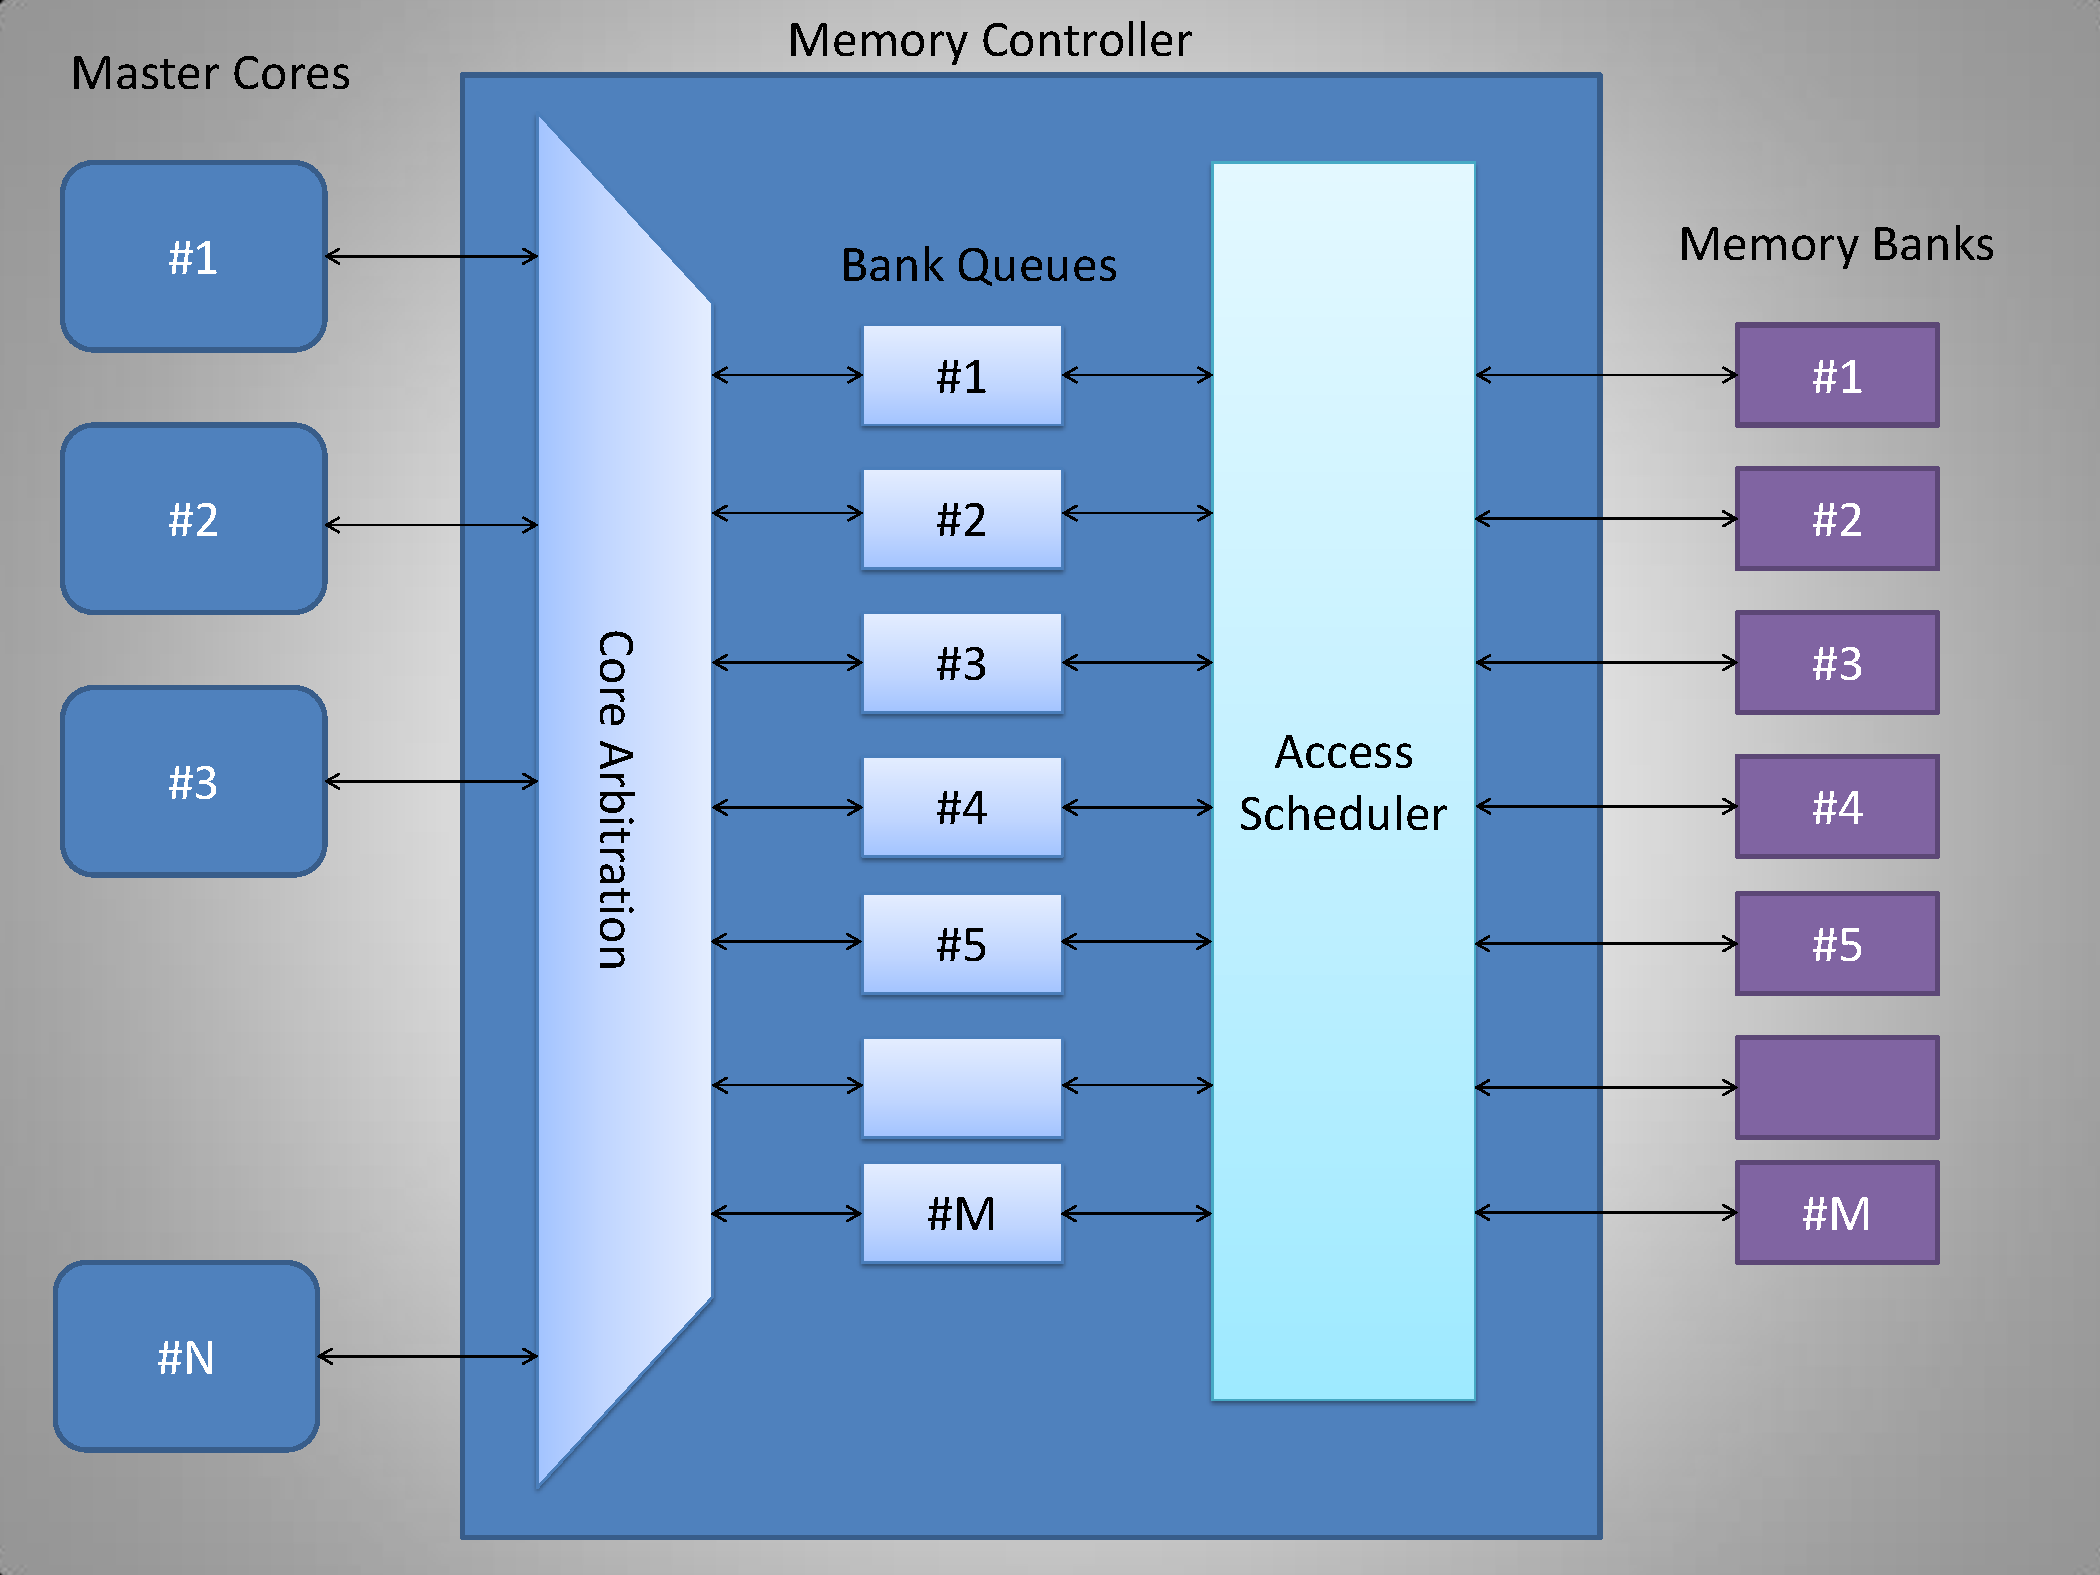
\includegraphics[width=0.7\linewidth]{fig/controllerArchitecture.pdf}
% \caption{
% {Architecture of Memory Controller} }
% \label{fig:pseudo-code}
% \end{figure}
% %-------------------------
The following three stages are illustrated in Figure~\ref{fig:multicore_arch}:
\begin{itemize}
\item \textbf{Core arbiter:~}Every clock cycle, the \textit{core arbiter} receives up to one request from each core which it stores in an internal queue. The core arbiter attempts to push these request to the appropriate bank queue. If it detects that the destination bank queue is full, the controller signals that the core is busy which stalls the core. The core arbiter also arranges the requests stored in its internal queue using a two-step priority order mechanism: first by Quality of Service (QoS) and then breaking ties with round-robin scheduling.

\item \textbf{Bank queues:~}Each data bank has a corresponding \textit{read queue} and \textit{write queue}.  The core arbiter sends memory requests to the bank queues until the queues are full. In our simulations, we use a bank queue depth of 10. There is also an additional queue which holds special requests such as memory refresh requests.

\item \textbf{Access scheduler:~}Every memory cycle, the \textit{access scheduler} chooses to serve read requests or write requests, algorithmically determining which requests in the bank queues it will schedule. The scheduling algorithms the access scheduler uses are called pattern builders. Depending on the current memory cycle's request type, the access scheduler invokes either the read or write pattern builder. A key design trade-off of the pattern builder algorithms is the relationship between the complexity of the algorithm and the number of requests the algorithm schedules.
\end{itemize}

We note that the core arbiter and bank queues should not differ much from those in a traditional uncoded memory controller. The access scheduler directly interacts with the memory banks, and therefore must be designed specifically for our coding schemes.


%-----------------------
\begin{figure}[tbp]
\centering
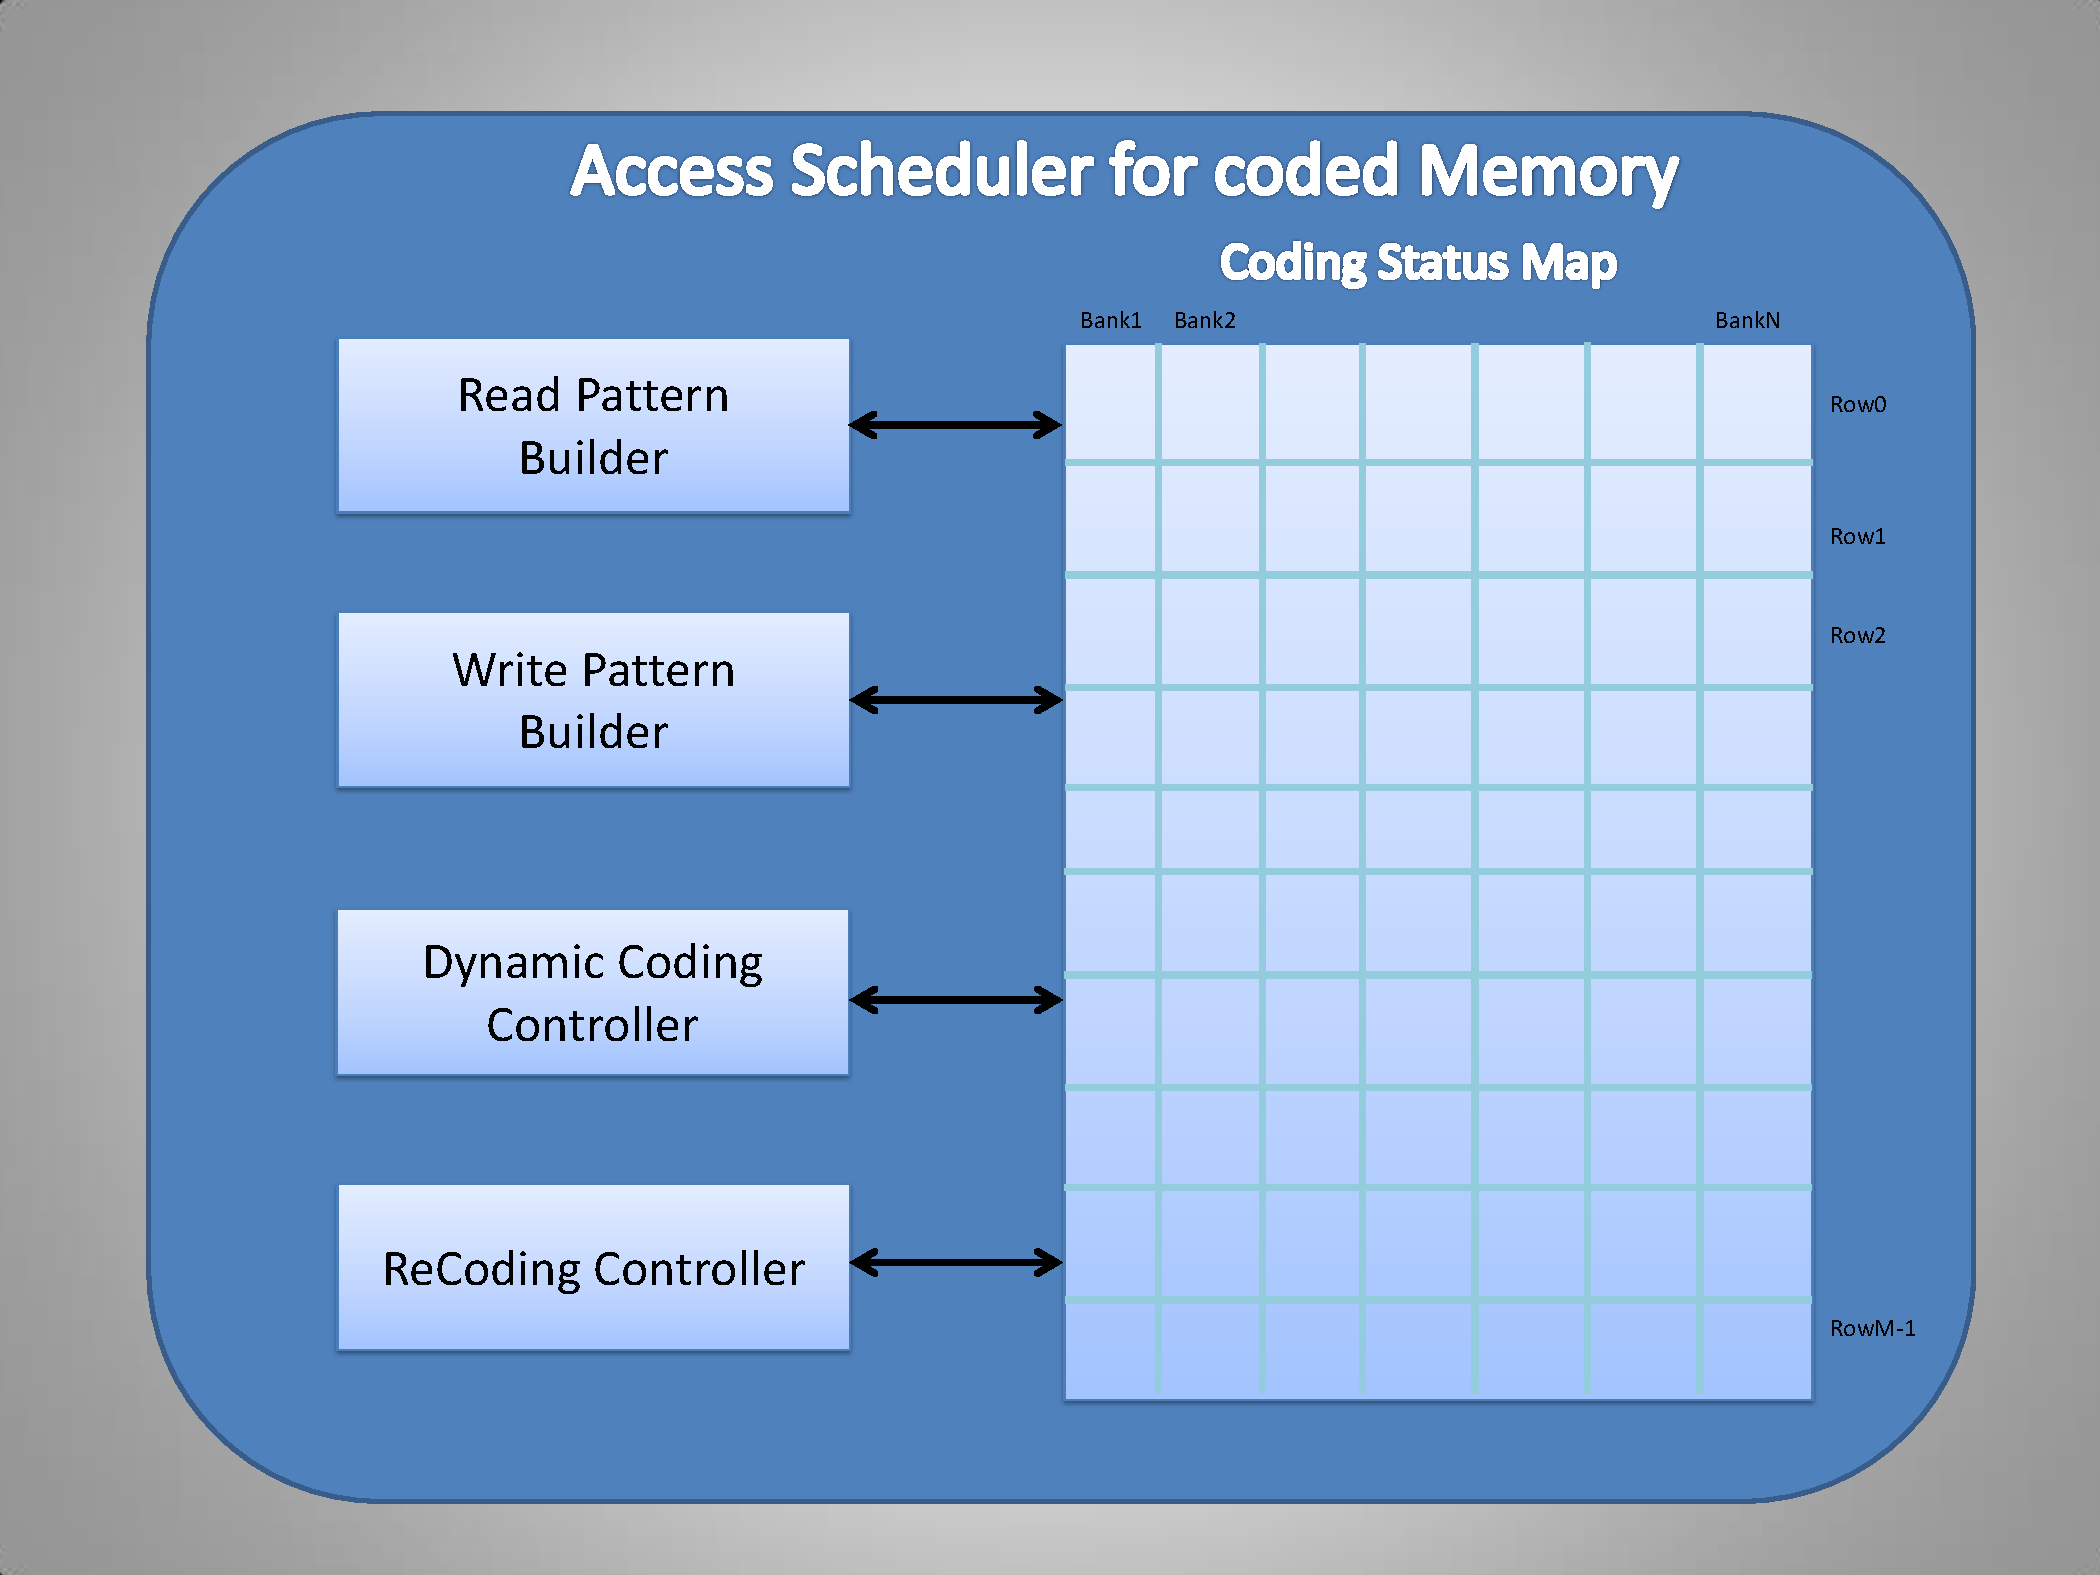
\includegraphics[width=0.7\linewidth]{fig/coded_access_scheduler.pdf}
\caption{
{Access scheduler for coded memory} }
\label{fig:coded_access_scheduler}
\end{figure}
%-------------------------
\subsection{Code Status Table}
\label{sec:codeStatusTable}
The code status table keeps track of the validity of data stored the data and parity banks. When a write is served to a row in a data bank, any parity bank which is constructed from the data bank will contain invalid data its corresponding row. Similarly, when the access scheduler serves a write to a parity bank, both the data bank which contains the memory address specified by the write request and any parity banks which utilizes that data bank will contain invalid data. The code status table keeps track of the locations of invalid data so the access scheduler does not erroneously serve read requests with stale data.

Figure~\ref{fig:coded_access_scheduler} depicts our implementation of the code status table. It contains an entry for every row in each data bank, which can take one of three values indicating 1) the data in both the data bank and parity banks is fresh, 2) the data bank contains the most recent data, or 3) one of the parity banks contains the most recent data. 
%It is not necessary for the code status table to know which parity bank a write request was served, because the dynamic coding unit described later in this section keeps track of this information. 
We assume that the elements of the code status table are accessible at a very fast rate. 


%{\color{red}
%This implementation of the code status table can be improved. This code status table does not keep track of the intermediate steps the access scheduler takes when rebuilding codes after a write is served. When rebuilding the memory in two parity banks after a data bank has been written to, it is likely that elements of one parity bank will be restored before the other. The restored parity bank is ready to serve more memory requests using the rebuilt row, but the code status table will indicate that all the parity banks are unavailable until all parity banks are restored. Full knowledge of the status of all data and parity banks allows the access scheduler to serve more requests in some scenarios. \Matt{is this example necessary? Is the tangent worth the insight?}
%}

%-----------------------
\begin{figure}[t!]
	%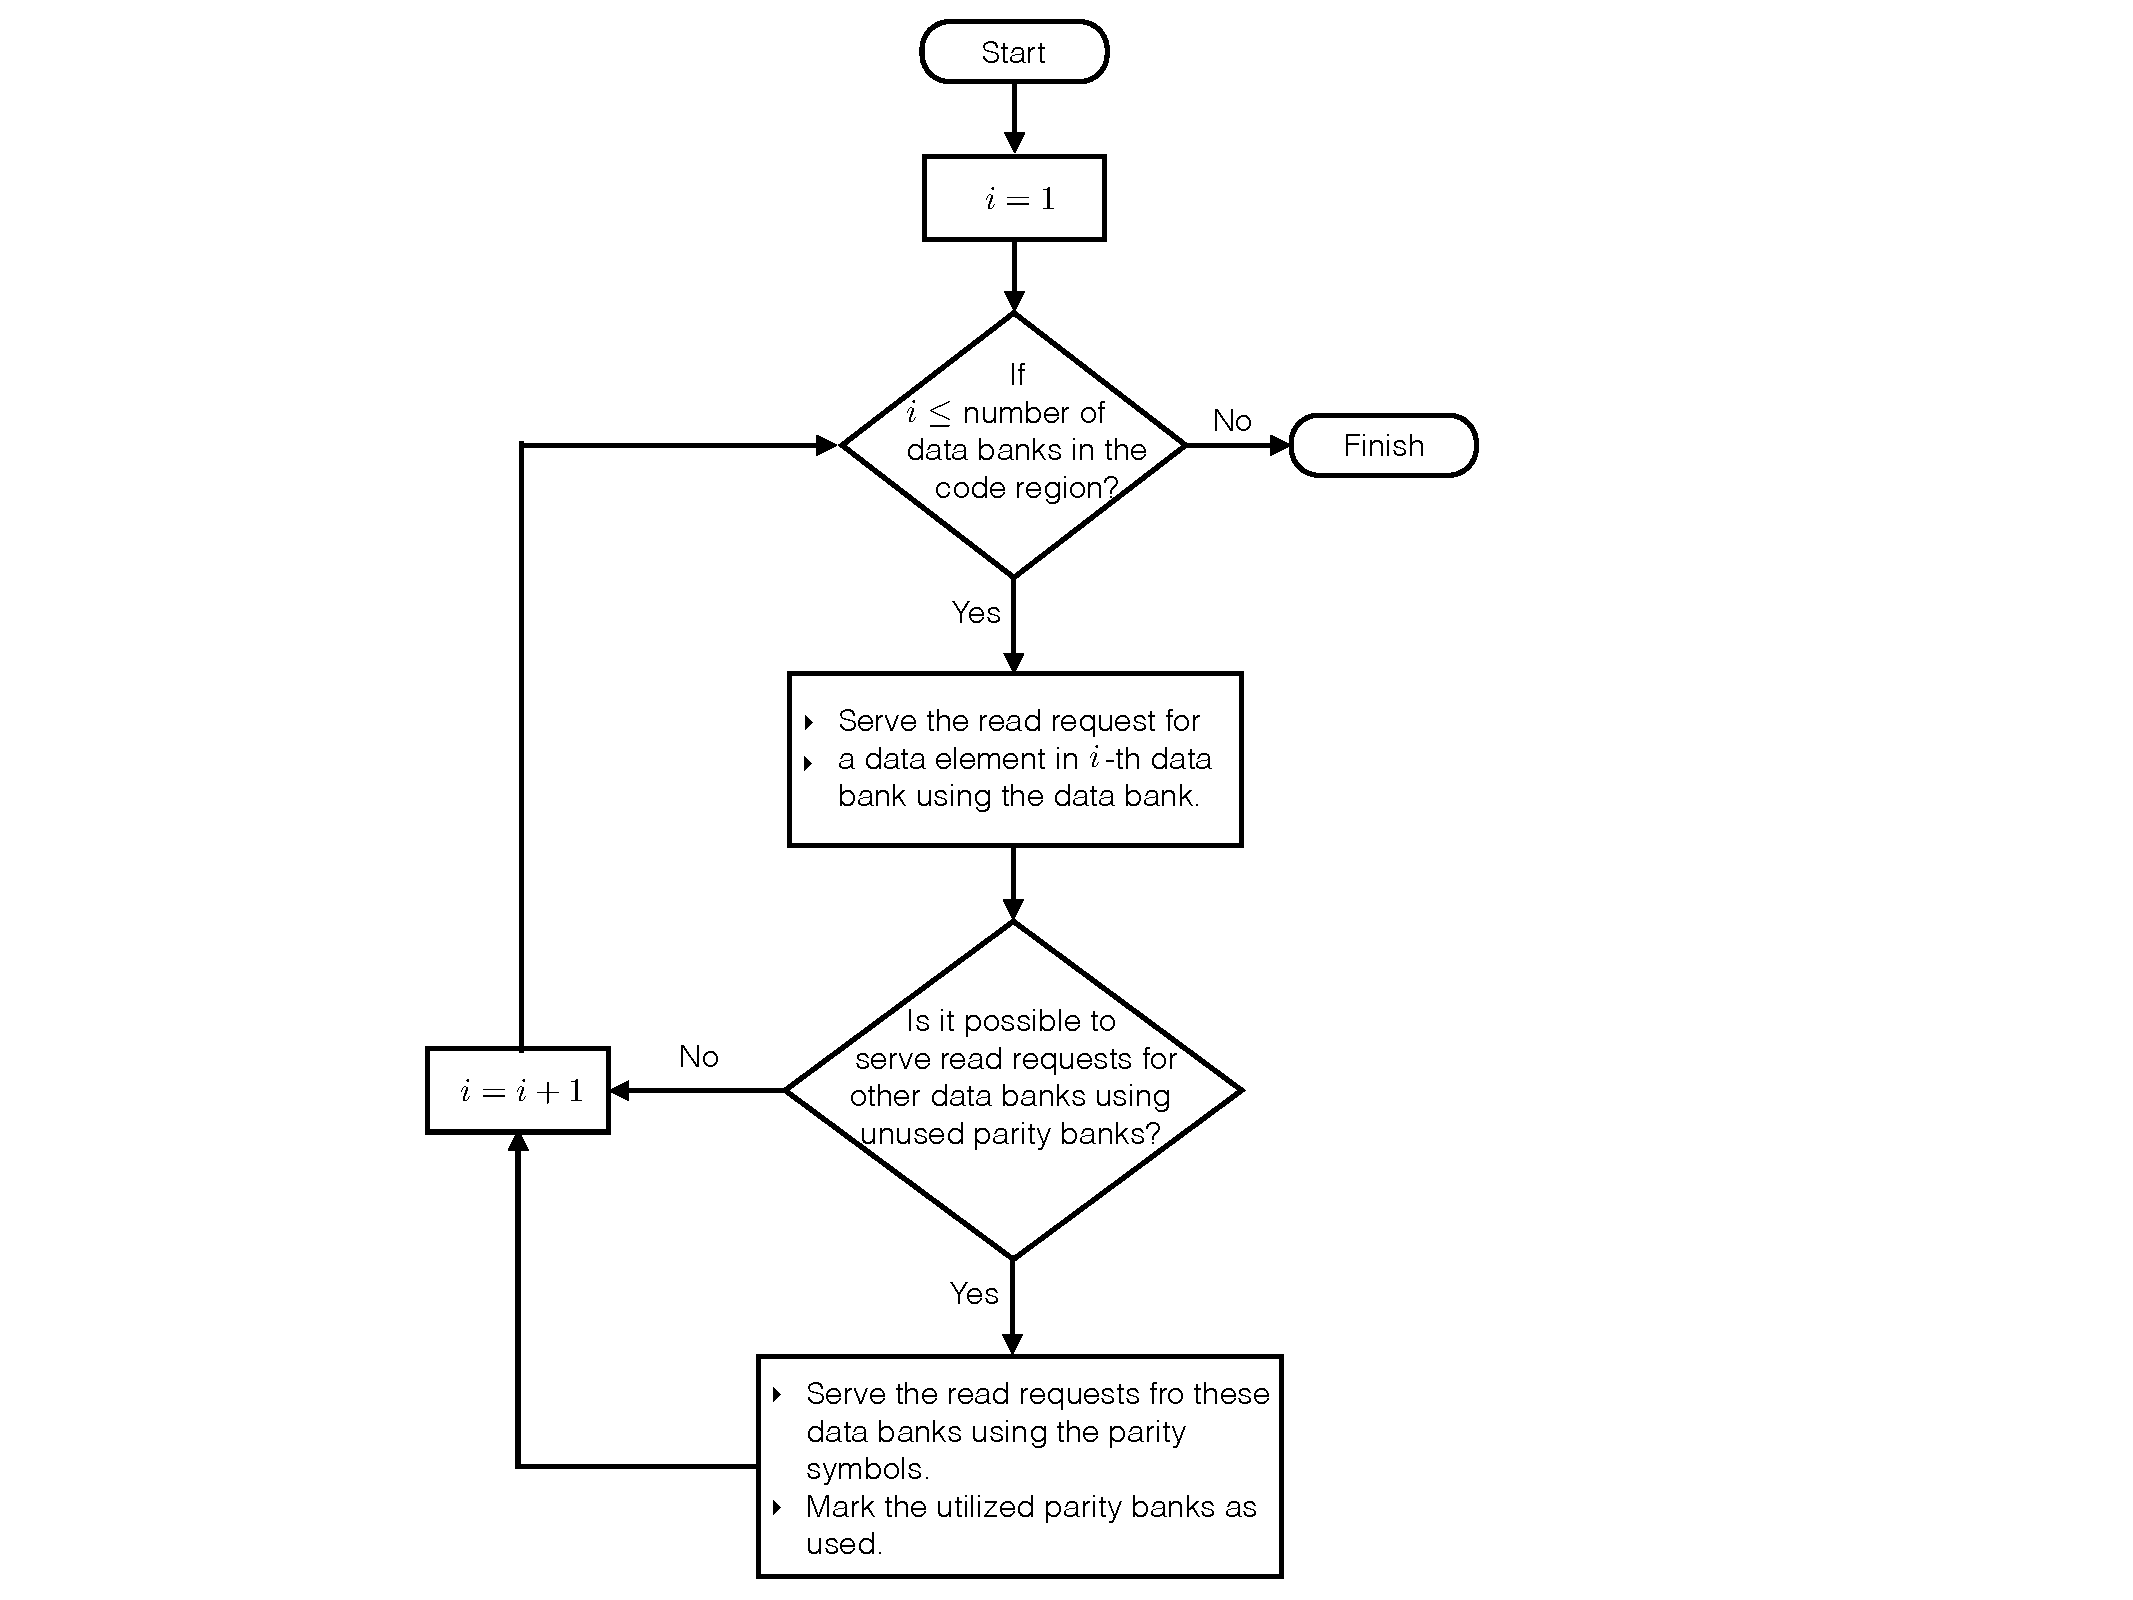
\includegraphics[width=0.9\linewidth]{fig/Read-algo.pdf}
	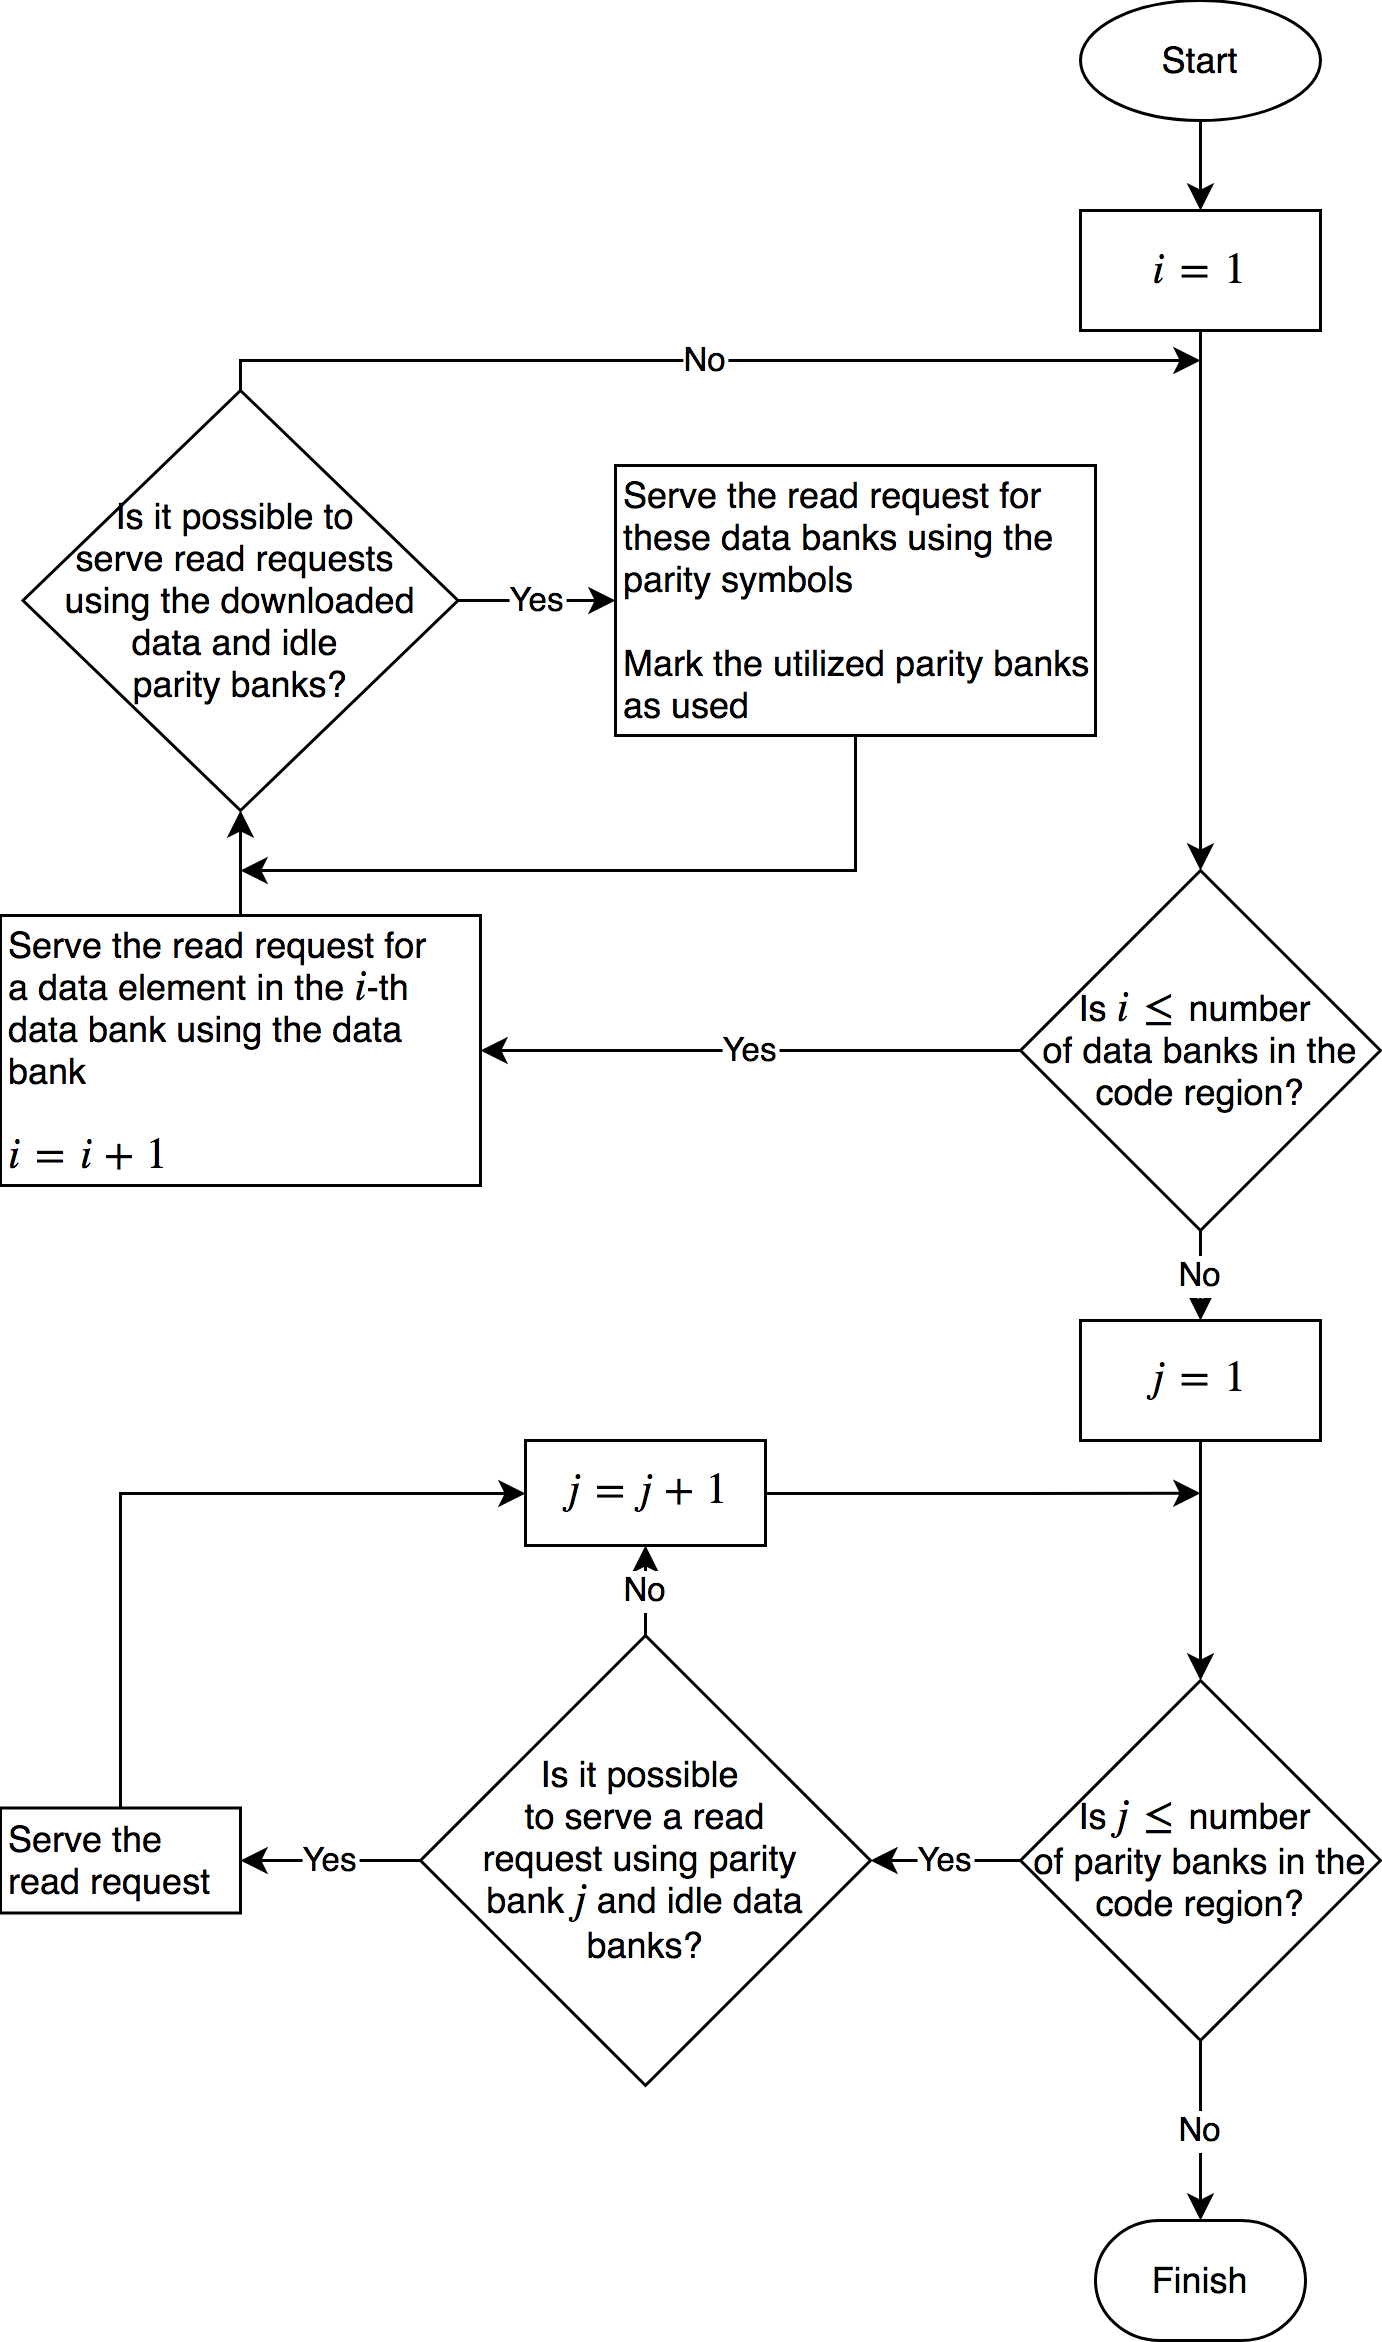
\includegraphics[width=0.6\linewidth]{fig/read_pattern_algo.png}
	\caption{{Description of the algorithm to build a read request pattern to be served in a given memory cycle.}}
	\label{fig:readAlgo}
\end{figure}
%-------------------------
%-----------------------
\begin{figure}[htbp]
	\centering
	%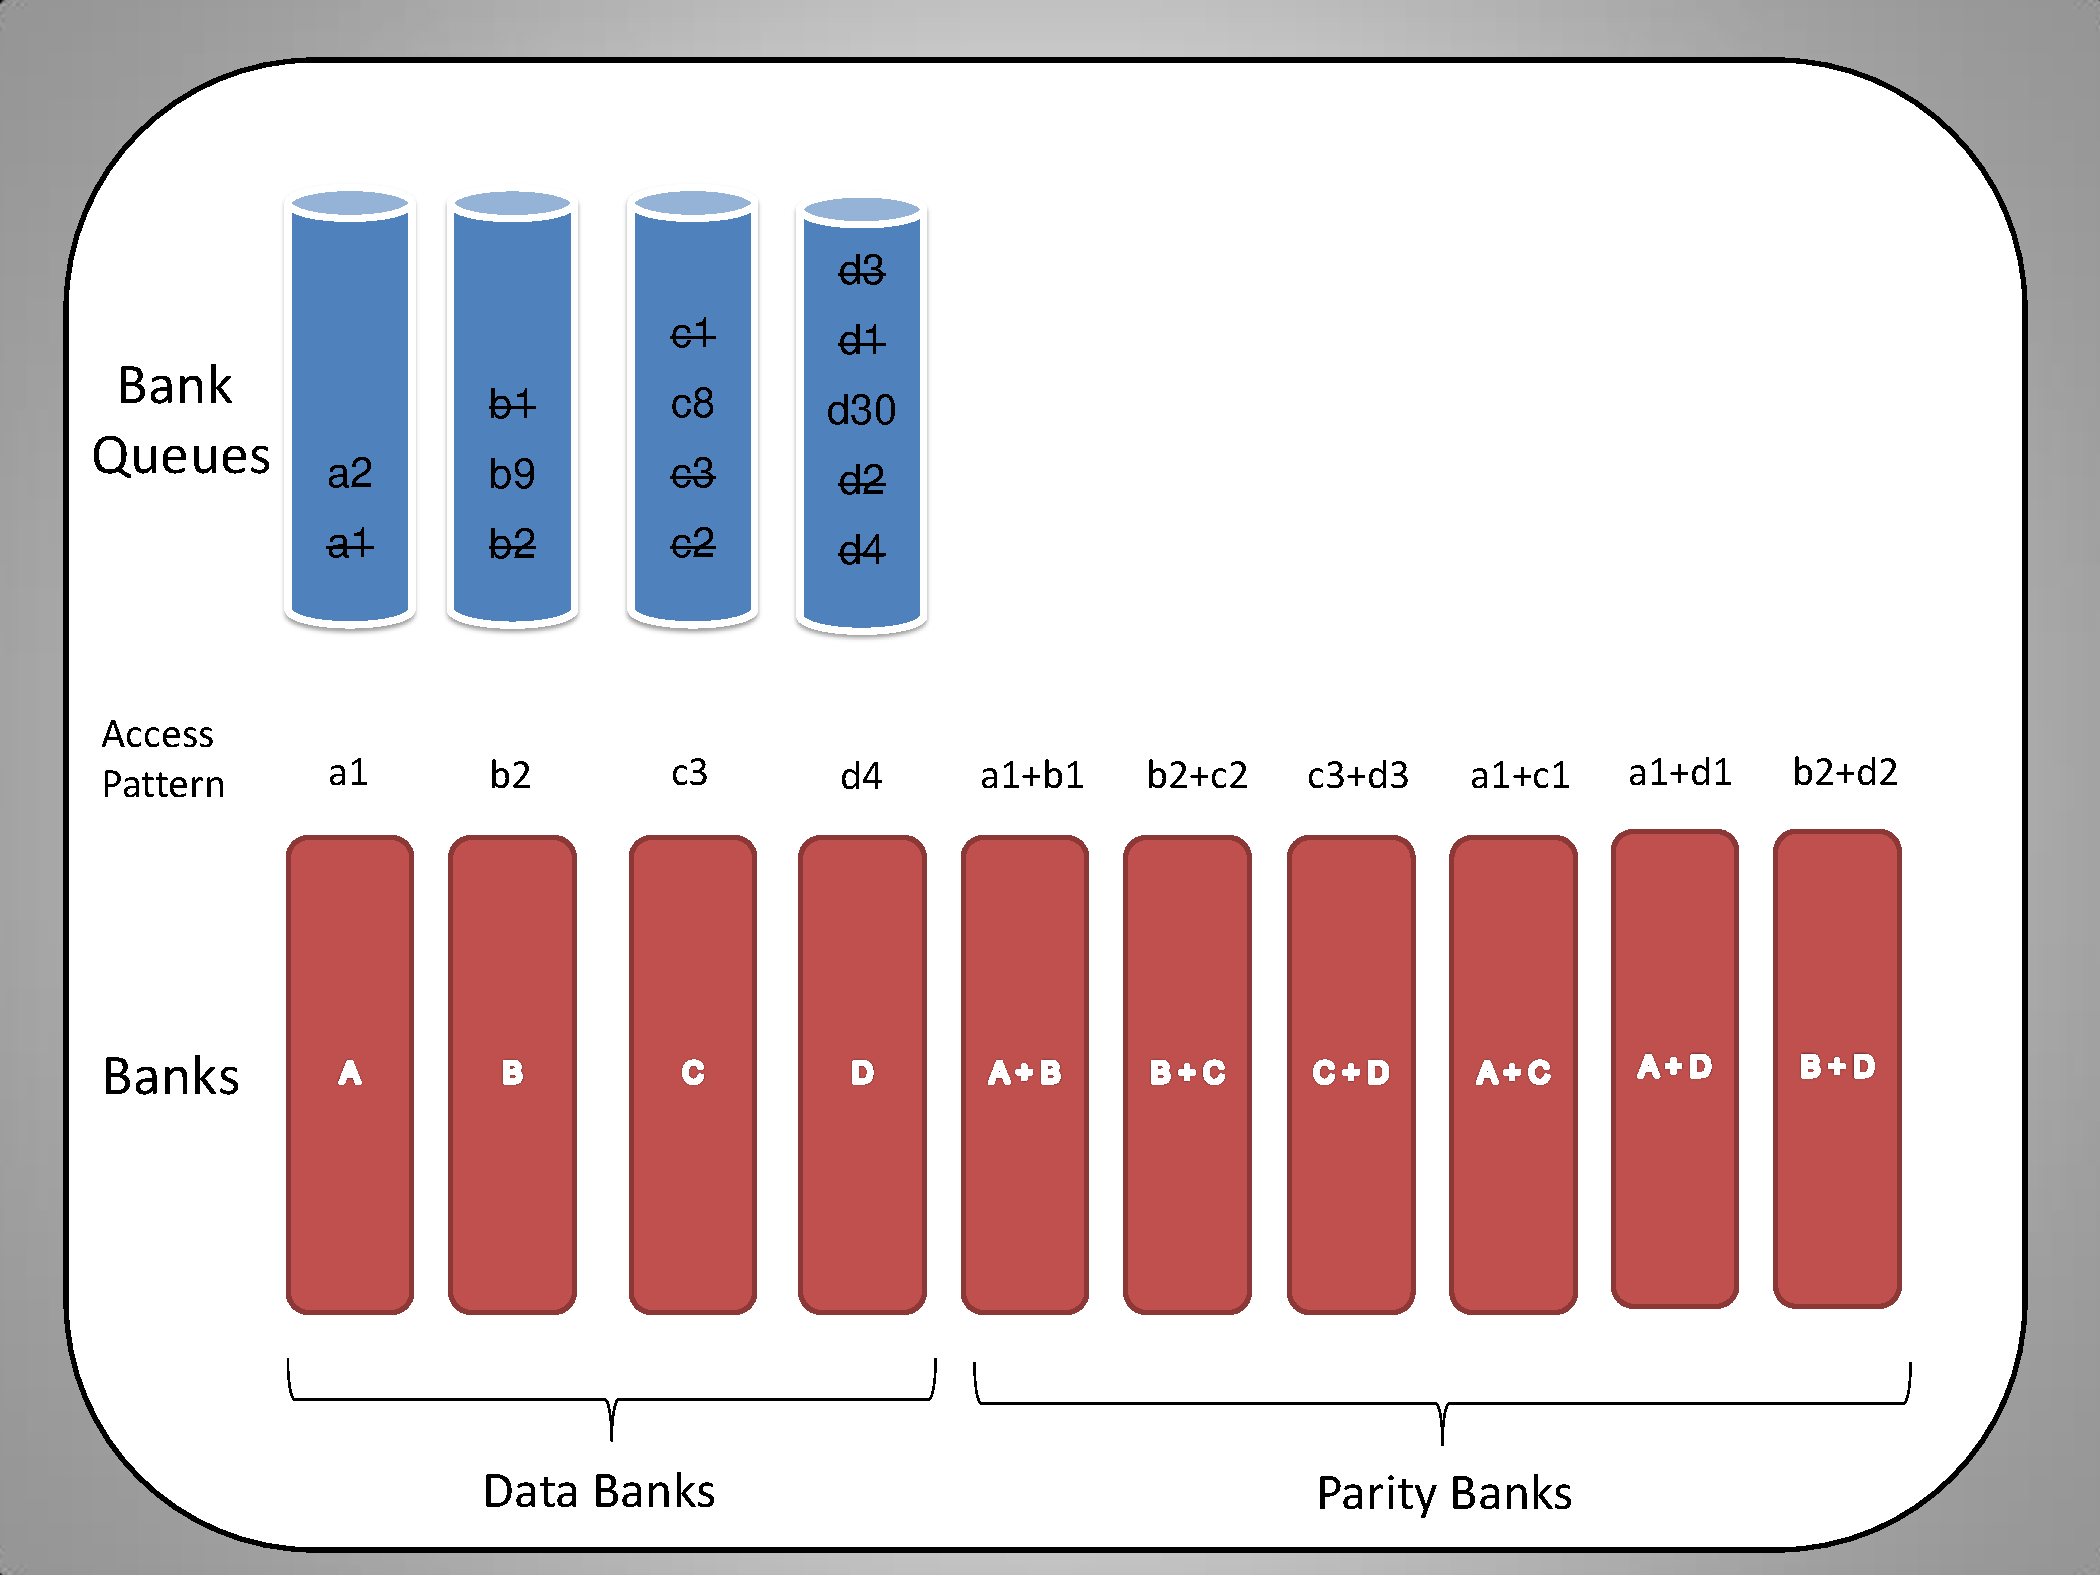
\includegraphics[width=0.7\linewidth]{fig/readAlgoAccessPattern.pdf}
	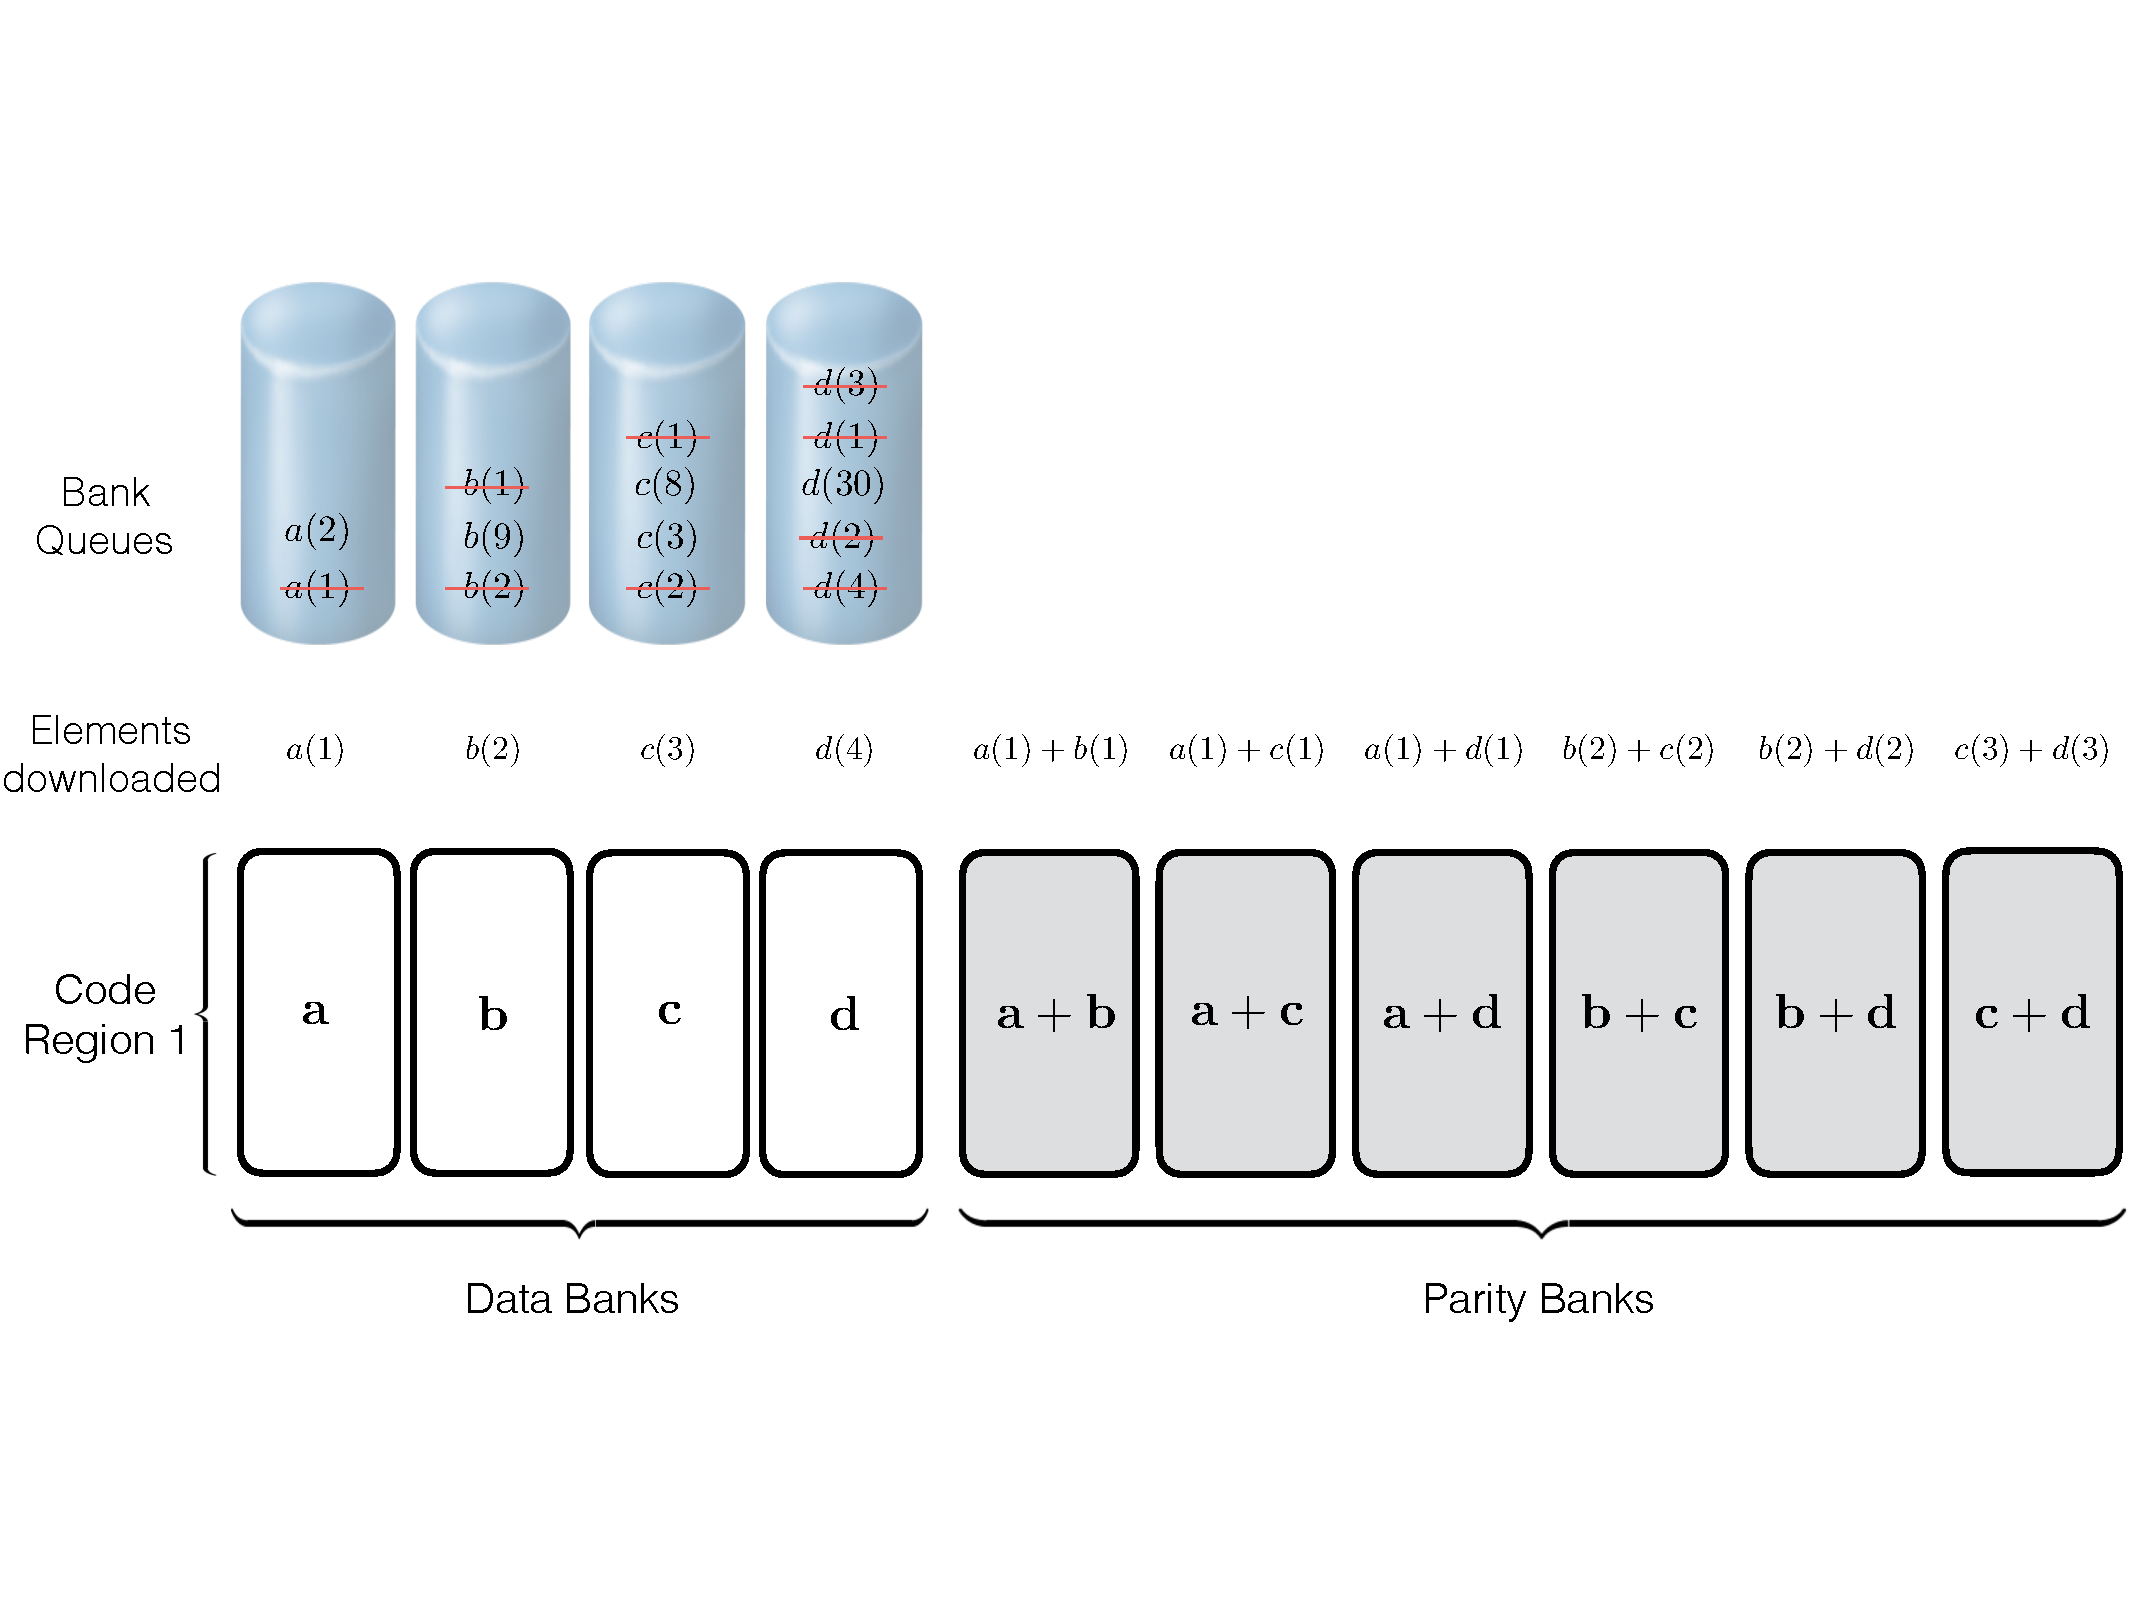
\includegraphics[width=0.96\linewidth]{fig/Read-Algo-Example.pdf}
	\caption{{Illustration of the algorithm to build a read request pattern to be served in a given memory cycle. All the read requests associated with the strikethrough elements are scheduled to be served in a given memory cycle. The figure also shows the elements downloaded from all the memory banks in order to serve these read requests.}}
	\label{fig:readAlgoAccessPattern}
\end{figure}
%------------------------
%\subsection{Read Algorithm for Coded Memory system}
\subsection{Read pattern builder}
\label{sec:readCodingAlgo}


The access scheduler uses the read pattern builder algorithm to determine which requests to serve using parity and which to use data banks. The read pattern builder selects which memory requests to serve and determines how requests served by parity banks will be decoded. The algorithm is designed to serve many read requests in a single memory cycle. Figure~\ref{fig:readAlgo} shows our implementation of the read pattern builder.

Figure~\ref{fig:readAlgoAccessPattern} shows an example read pattern constructed by our algorithm. First, $a(1)$ is marked to be read from data bank $\mathbf{a}$. Then the algorithm looks through banks $\mathbf{b}$, $\mathbf{c}$, and $\mathbf{d}$ for requests for rows $b(1)$, $c(1)$, or $d(1)$ because these symbols can be decoded from a parity bank using the $a(1)$ symbol. In this scenario all three are present in the bank queues and are served using parity banks. Symbols equal to  $a(1) + b(1)$, $a(1) + c(1)$, and $a(1) + d(1)$ are all downloaded from parity banks and decoded with $a(1)$. Next, $b(2$) is read from a data bank. Similar to before, $c(2)$ and $d(2)$ are served by downloading $b(2) + c(2)$ and $b(2) + d(2)$ symbols from the parity banks. Again as before, $c(3)$ is read from data bank and $d(3)$ is decoded using $c(3)$ and $c(3) + d(3)$. Finally, $d(4)$ is read from a data bank.

\begin{remark}
By increasing the number of read requests per cycle, we increase the risk of having out-of-order execution of memory access requests on the same core. We assume that the code arbiter only admits requests into the bank queues if they can be immediately served without introducing harmful out-of-order execution.


\end{remark}
\ignore{
%-----------------------
\begin{figure}[htbp]
\centering
	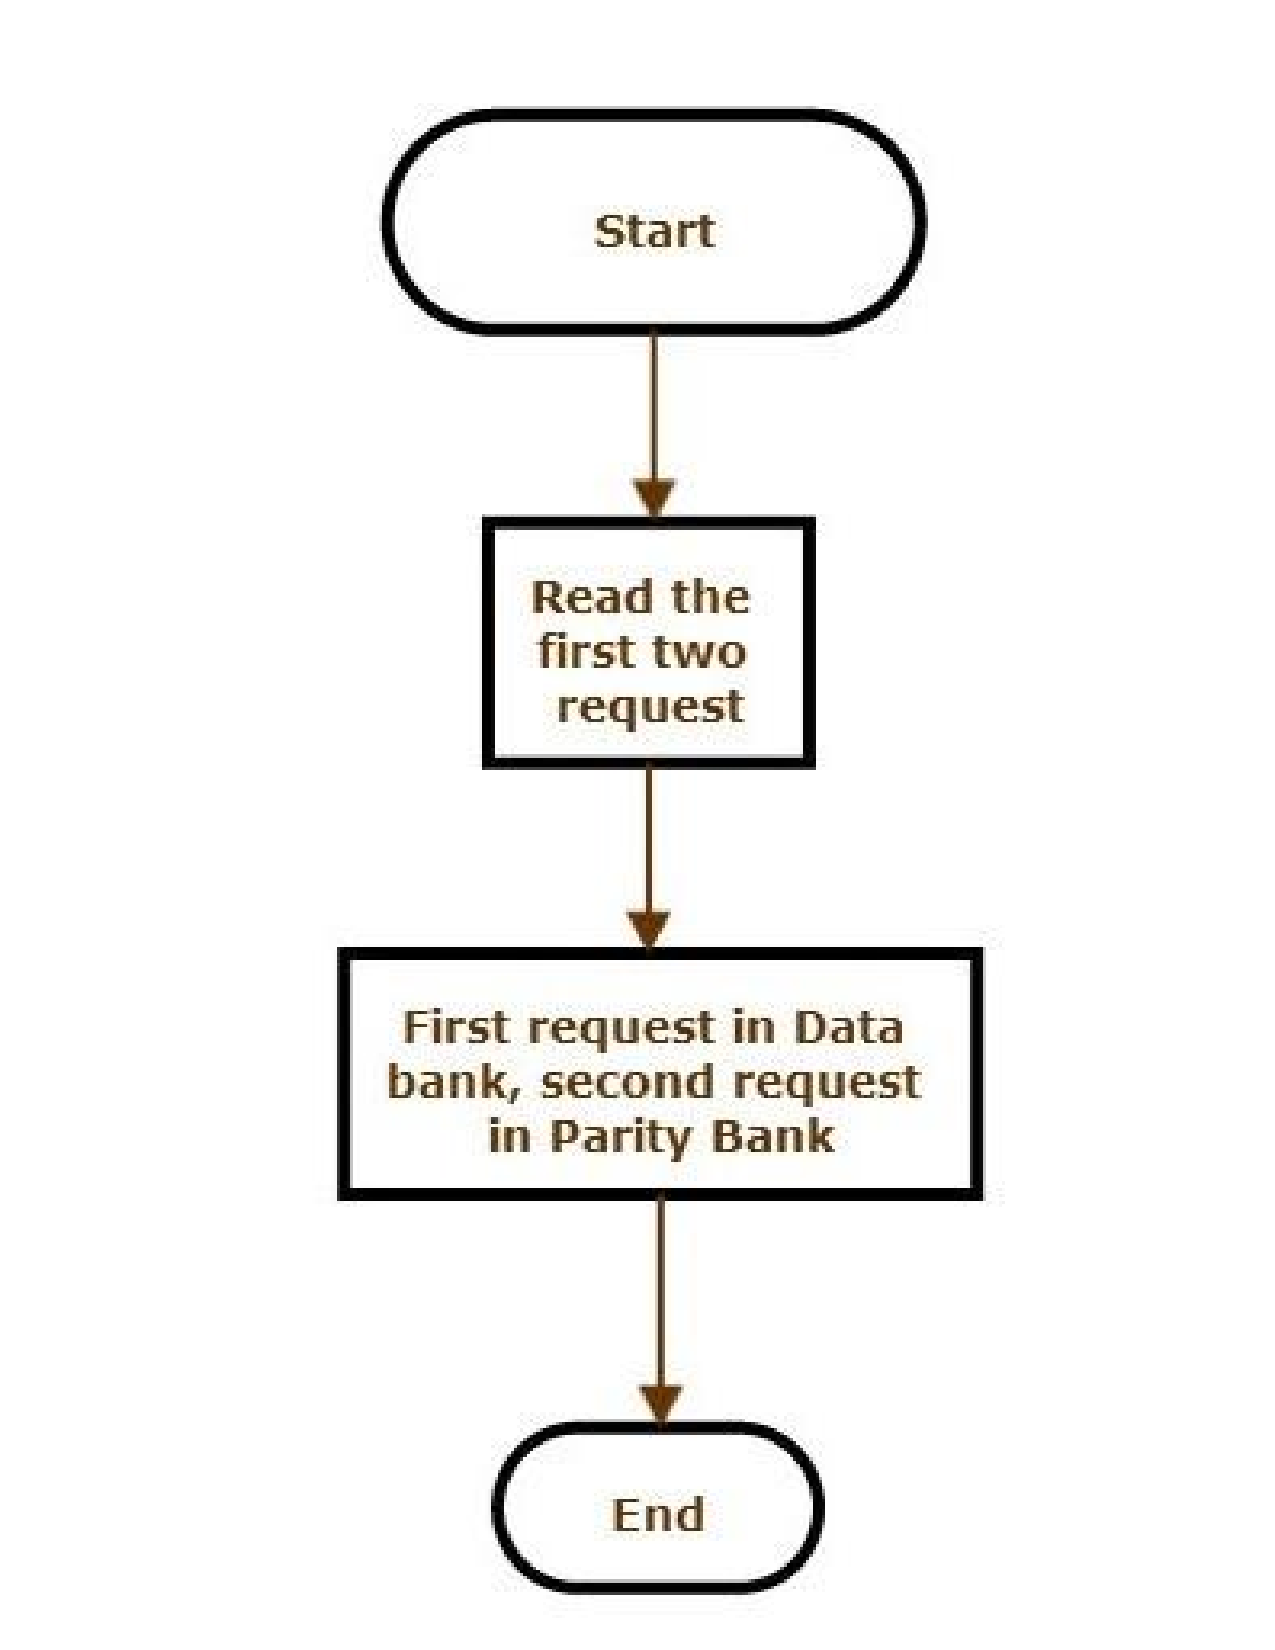
\includegraphics[width=0.6\linewidth]{fig/writealgo.pdf}
	\caption{{\bf Flowchart of Write Algorithm}}
	\label{fig:writeAlgo}
\end{figure}
%-------------------------
%\ignore{
\begin{itemize}
\item Write about how we solve the out of order look ahead problem. If we solve 
	it at all ????
\end{itemize}
}
%\subsection{Write Algorithm for Coded Memory system}
\subsection{Write pattern builder}
\label{sec:writeCodingAlgo}
Parity banks allow the memory controller to serve additional write requests per cycle. When multiple writes target a single bank, it can commit some of them to parity banks. The access scheduler implements a write pattern builder algorithm to determine which write requests to schedule in a single memory cycle. Figure~\ref{fig:writeFlow} illustrates our implementation of the write pattern builder. Only when the write bank queues are nearly full does the access scheduler execute the write pattern builder algorithm. 


%-----------------------
\begin{figure}[htbp]
\centering
	\includegraphics[width=0.6\linewidth]{fig/write_pattern_algo.png}
	\caption{{ Flowchart of write pattern builder}}
	\label{fig:writeFlow}
\end{figure}
%-------------------------


Figure~\ref{fig:writeAlgoAccessPattern} shows an example write pattern produced by our algorithm. Parity banks increase the maximum number of write requests from $4$ to $10$. Note that an element which is addressed to row $n$ in a data bank can only be written to the corresponding row $n$ in the parity banks. In this scenario, the write queues for every data bank are full. The controller takes $2$ write requests from each queue and schedules one to the queue's target data bank and the other to a parity bank. The controller also updates the code status table.

{\color{red}
Figure~\ref{fig:writeAlgoAccessPattern} also demonstrates how the code status table changes to reflect the freshness of the elements in the data and parity banks. Here, the 00 status indicates that all elements are updated. The 01 status indicates that the data banks contain fresh elements and the elements in the parity banks must be recoded. The 10 status indicates that the parity banks contain fresh elements, and that both data banks and parity banks must be updated.
}

%-----------------------
\begin{figure}[t!]
\centering
         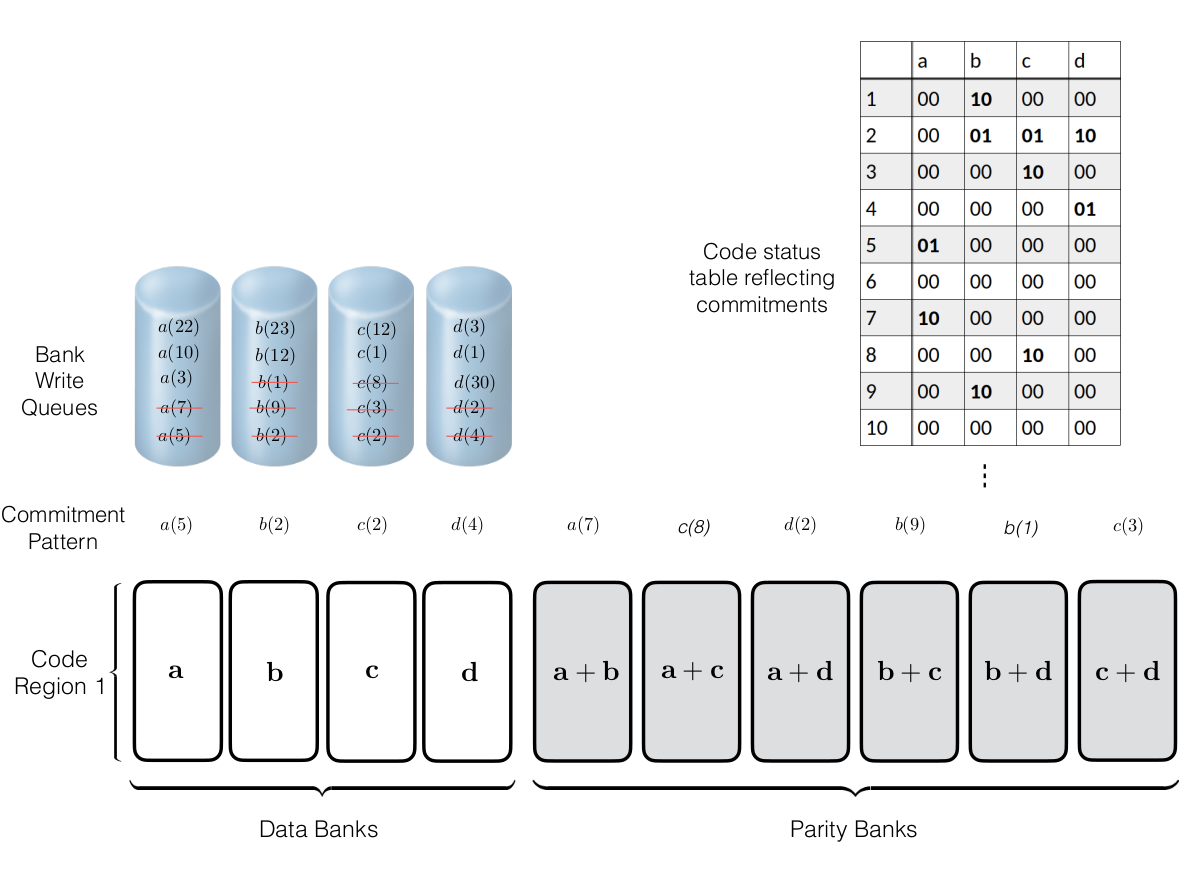
\includegraphics[width=\linewidth]{fig/Write-Algo-Example.png}
	\caption{The behavior of the write pattern builder on a 4-bank memory system}
	\label{fig:writeAlgoAccessPattern}
\end{figure}
%-------------------------
\subsection{ReCoding unit}
\label{sec:recoding}
After a write request has been served, the stale data in the parity (or data) banks must be replaced. The \textit{ReCoding Unit} accomplishes this with a queue of {\em recoding requests}. Every time a write is served, recoding requests are pushed on to the queue indicating which data and parity banks contain stale elements, as well as the bank which generated the recoding request. Requests also contain the current cycle number so that the ReCoding Unit may prioritize older requests. Appendix

\subsection{Dynamic Coding}
\label{sec:dynamicCoding}
To reduce memory overhead $\alpha$, parity banks are designed to be smaller than data banks. The dynamic coding block maintains codes for the most heavily accessed memory subregions, so that parity banks are utilized more often.
%
%\subsubsection{Encoder Design}
%There are many possible implementations of the dynamic coding unit. The design described here is used in the simulator used to generate the results described in sections 5 and 6.
%
The {\em dynamic coding} block partitions each memory bank into $\lceil\frac{1}{r}\rceil$ regions. The block can select up to $\frac{\alpha}{r} - 1$ regions to be encoded in the parity banks. A single region is reserved to allow encoding of a new region.

Every $T$ cycles, the dynamic coding unit chooses the $\frac{\alpha}{r} - 1$ regions with the greatest number of memory accesses. The dynamic coding unit will then encode these regions in the parity banks. If all the selected regions are already encoded, the unit does nothing. Otherwise, the unit begins encoding the most accessed region. Once the dynamic coding unit is finished encoding a new region, the region becomes available for use by the rest of the memory controller. A memory region of length $r$ is reserved by the dynamic coding unit for constructing new encoded regions, and a memory region of length $\alpha - r$ is reserved for active encoded regions. If the memory ceiling $\alpha - r$ is reached when a new memory region is encoded, the unit evicts the least frequently used encoded region.

\subsection{Prefetching Codes}
\label{sec:prefetching}
Dynamic coding works best when the most heavily accessed regions of memory vary little to none over time. When the memory access trend is not static, the proposed memory system can benefit from anticipating structured (\textit{e.g.} sequential) memory accesses. Therefore, our design includes a prefetcher which detects sequential memory accesses and exploits idle memory banks to potentially serve future memory requests. The prefetcher prioritizes long sequential memory accesses as motivation for performing an anticipatory read. Because of the speculative nature of the prefetcher, it is given the lowest priority of all the components in the access scheduler. It only schedules a memory access if all the other units have not done so first. 
\Ethan{More details here?}